% Template for PLoS
% Version 3.6 Aug 2022
%
% % % % % % % % % % % % % % % % % % % % % %
%
% -- IMPORTANT NOTE
%
% This template contains comments intended 
% to minimize problems and delays during our production 
% process. Please follow the template instructions
% whenever possible.
%
% % % % % % % % % % % % % % % % % % % % % % % 
%
% Once your paper is accepted for publication, 
% PLEASE REMOVE ALL TRACKED CHANGES in this file 
% and leave only the final text of your manuscript. 
% PLOS recommends the use of latexdiff to track changes during review, as this will help to maintain a clean tex file.
% Visit https://www.ctan.org/pkg/latexdiff?lang=en for info or contact us at latex@plos.org.
%
%
% There are no restrictions on package use within the LaTeX files except that no packages listed in the template may be deleted.
%
% Please do not include colors or graphics in the text.
%
% The manuscript LaTeX source should be contained within a single file (do not use \input, \externaldocument, or similar commands).
%
% % % % % % % % % % % % % % % % % % % % % % %
%
% -- FIGURES AND TABLES
%
% Please include tables/figure captions directly after the paragraph where they are first cited in the text.
%
% DO NOT INCLUDE GRAPHICS IN YOUR MANUSCRIPT
% - Figures should be uploaded separately from your manuscript file. 
% - Figures generated using LaTeX should be extracted and removed from the PDF before submission. 
% - Figures containing multiple panels/subfigures must be combined into one image file before submission.
% For figure citations, please use "Fig" instead of "Figure".
% See http://journals.plos.org/plosone/s/figures for PLOS figure guidelines.
%
% Tables should be cell-based and may not contain:
% - spacing/line breaks within cells to alter layout or alignment
% - do not nest tabular environments (no tabular environments within tabular environments)
% - no graphics or colored text (cell background color/shading OK)
% See http://journals.plos.org/plosone/s/tables for table guidelines.
%
% For tables that exceed the width of the text column, use the adjustwidth environment as illustrated in the example table in text below.
%
% % % % % % % % % % % % % % % % % % % % % % % %
%
% -- EQUATIONS, MATH SYMBOLS, SUBSCRIPTS, AND SUPERSCRIPTS
%
% IMPORTANT
% Below are a few tips to help format your equations and other special characters according to our specifications. For more tips to help reduce the possibility of formatting errors during conversion, please see our LaTeX guidelines at http://journals.plos.org/plosone/s/latex
%
% For inline equations, please be sure to include all portions of an equation in the math environment.  For example, x$^2$ is incorrect; this should be formatted as $x^2$ (or $\mathrm{x}^2$ if the romanized font is desired).
%
% Do not include text that is not math in the math environment. For example, CO2 should be written as CO\textsubscript{2} instead of CO$_2$.
%
% Please add line breaks to long display equations when possible in order to fit size of the column. 
%
% For inline equations, please do not include punctuation (commas, etc) within the math environment unless this is part of the equation.
%
% When adding superscript or subscripts outside of brackets/braces, please group using {}.  For example, change "[U(D,E,\gamma)]^2" to "{[U(D,E,\gamma)]}^2". 
%
% Do not use \cal for caligraphic font.  Instead, use \mathcal{}
%
% % % % % % % % % % % % % % % % % % % % % % % % 
%
% Please contact latex@plos.org with any questions.
%
% % % % % % % % % % % % % % % % % % % % % % % %

\documentclass[10pt,letterpaper]{article}
\usepackage[top=0.85in,left=2.75in,footskip=0.75in]{geometry}

% amsmath and amssymb packages, useful for mathematical formulas and symbols
\usepackage{amsmath,amssymb}

% Use adjustwidth environment to exceed column width (see example table in text)
\usepackage{changepage}

% textcomp package and marvosym package for additional characters
\usepackage{textcomp,marvosym}

% cite package, to clean up citations in the main text. Do not remove.
\usepackage{cite}

% Use nameref to cite supporting information files (see Supporting Information section for more info)
\usepackage{nameref,hyperref}
\usepackage[normalem]{ulem}
% line numbers
\usepackage[right]{lineno}

% ligatures disabled
\usepackage[nopatch=eqnum]{microtype}
\DisableLigatures[f]{encoding = *, family = * }

% color can be used to apply background shading to table cells only
\usepackage[table]{xcolor}

% array package and thick rules for tables
\usepackage{array}

% create "+" rule type for thick vertical lines
\newcolumntype{+}{!{\vrule width 2pt}}

% create \thickcline for thick horizontal lines of variable length
\newlength\savedwidth
\newcommand\thickcline[1]{%
  \noalign{\global\savedwidth\arrayrulewidth\global\arrayrulewidth 2pt}%
  \cline{#1}%
  \noalign{\vskip\arrayrulewidth}%
  \noalign{\global\arrayrulewidth\savedwidth}%
}

% \thickhline command for thick horizontal lines that span the table
\newcommand\thickhline{\noalign{\global\savedwidth\arrayrulewidth\global\arrayrulewidth 2pt}%
\hline
\noalign{\global\arrayrulewidth\savedwidth}}


% Remove comment for double spacing
%\usepackage{setspace} 
%\doublespacing

% Text layout
\raggedright
\setlength{\parindent}{0.5cm}
\textwidth 5.25in 
\textheight 8.75in

% Bold the 'Figure #' in the caption and separate it from the title/caption with a period
% Captions will be left justified
\usepackage[aboveskip=1pt,labelfont=bf,labelsep=period,justification=raggedright,singlelinecheck=off]{caption}

\renewcommand{\figurename}{Fig}

% Use the PLoS provided BiBTeX style
\bibliographystyle{plos2015}

% Remove brackets from numbering in List of References
\makeatletter
\renewcommand{\@biblabel}[1]{\quad#1.}
\makeatother



% Header and Footer with logo
\usepackage{lastpage,fancyhdr,graphicx}
\usepackage{epstopdf}
%\pagestyle{myheadings}
\pagestyle{fancy}
\fancyhf{}
%\setlength{\headheight}{27.023pt}
%\lhead{\includegraphics[width=2.0in]{PLOS-submission.eps}}
\rfoot{\thepage/\pageref{LastPage}}
\renewcommand{\headrulewidth}{0pt}
\renewcommand{\footrule}{\hrule height 2pt \vspace{2mm}}
\fancyheadoffset[L]{2.25in}
\fancyfootoffset[L]{2.25in}
\lfoot{\today}

%% Include all macros below

\newcommand{\lorem}{{\bf LOREM}}
\newcommand{\ipsum}{{\bf IPSUM}}

%% END MACROS SECTION


\begin{document}
\vspace*{0.2in}

% Title must be 250 characters or less.
\begin{flushleft}
{\Large
\textbf\newline{Untangling temporal signal for calibrating the molecular clock of microbes} % Please use "sentence case" for title and headings (capitalize only the first word in a title (or heading), the first word in a subtitle (or subheading), and any proper nouns).
}
\newline
% Insert author names, affiliations and corresponding author email (do not include titles, positions, or degrees).
\\
John H Tay\textsuperscript{1},
Arthur Kocher\textsuperscript{2,3},
Sebastian Duchene\textsuperscript{1,2,*},
\\
\bigskip
\textbf{1} Peter Doherty Institute for Infection and Immunity, Department of Microbiology and Immunology, University of Melbourne, Melbourne, Australia
\\
\textbf{2} Pending pending.
\\
\textbf{3} Department of Computational Biology, Institut Pasteur, Paris, France
\\
\bigskip

% Insert additional author notes using the symbols described below. Insert symbol callouts after author names as necessary.
% 

% \textcurrency b Insert second current address 
% \textcurrency c Insert third current address

% Use the asterisk to denote corresponding authorship and provide email address in note below.
* sduchene@pasteur.fr

\end{flushleft}
% Please keep the abstract below 300 words
\section*{Abstract}
Our understanding of the evolution of many microbes has been revolutionised by the molecular clock, a statistical tool to infer evolutionary rates and timescales. The fundamental assumption of molecular clock models is that the rate at which substitutions accumulate can be described by a statistical process. In all molecular clock models evolutionary rates and times are unidentifiable, and therefore 'calibration' information is essential to obtain estimates in calendar time.

For many microbes, the sequence sampling times themselves can be often used for calibration. Phylogenetic tests of temporal signal are often used to decide whether such calibrations are reliable. Critically, in addition to the calibration information, the full Bayesian phylogenetic model also includes the molecular clock model and a branching process (tree prior). As a result, there are multiple sources of information that are difficult to untangle.

We assessed temporal signal in three microbial data sets of human and animal diseases with a range of evolutionary characteristics and with ancient DNA sequences; \textit{Powassan virus} (POWV), the cholera bacetrium (\textit{Vibrio cholerae}), and the syphilis bacterium (\textit{Treponema palladium.}). We found that the tree prior can have a substantial impact on whether temporal signal is detected. To investigate this problem we conducted extensive simulations and calculated the sensitivity and specificity of these tests under several tree priors.  Highly informative sequence data sets are generally robust to the tree prior. However, in data sets with low information content, choosing a prior that is highly informative and inconsistent with the data can result in the false rejection of temporal signal. 

We demonstrate that prior sensitivity analyses and prior predictive simulations are an effective means to determine whether the prior is reasonable and to improve the detection of temporal signal and leverage the information that can be drawn from molecular sequence data sets.


% Please keep the Author Summary between 150 and 200 words
% Use first person. PLOS ONE authors please skip this step. 
% Author Summary not valid for PLOS ONE submissions.   
\section*{Author summary}
\textcolor{red}{Pending.}
\linenumbers

% Use "Eq" instead of "Equation" for equation citations.
\section*{Introduction}
Molecular sequence data have been essential to unravel the evolutionary history of many organisms. The molecular clock is a statistical tool that posits that molecular evolution, in the form of substitutions, follows a statistical process. For example, under the simplest molecular clock model, known as the strict clock, substitutions accumulate linearly over time along a lineage, such that the evolutionary rate is constant over time \cite{zuckerkandl1965evolutionary}. At the other end of the spectrum, relaxed molecular clocks allow every lineage in a phylogenetic tree to display a different evolutionary rate (\cite{drummond2006relaxed} and reviewed in \cite{ho2014molecular}). 

All molecular clock models have a fundamental limitation, where evolutionary rates and times are unidentifiable. That is, there exist an infinite number of combinations of evolutionary rates and times that are compatible with an amount of evolutionary divergence \cite{yang2006bayesian,dos2013unbearable}. For this reason, external information, known as a molecular clock calibration is necessary to produce estimates in calendar units. As a case in point, consider two sequences whose genetic divergence from their most recent common ancestor is 10 subs/site. In the absence of calibrating information it is impossible to know \textit{how rapidly} they evolve and \textit{when} they diverged. The calibration can be a known evolutionary rate, such as 1 subs/site/year, or a divergence date, such as 1 year before present. The genetic distance can be divided by the evolutionary rate to infer the divergence time to infer a time to the most recent common ancestor of 10 years, or the genetic distance can be divided by the divergence date to infer the evolutionary rate, 10/subs/site/year in this case.

The finding that some organisms accumulate substitutions in a measurable timescale prompted the use of sequence sampling times for calibration \cite{rodrigo1999coalescent, korber2000timing}. The motivation behind this practice is that sequence data collected at different points in time would have accumulated a corresponding number of substitutions. With the example above, a sequence collected six months of the common ancestor would have accumulated 5 subs/site (10 subs/site/year $\times$ 0.5 years = 5 subs/site), whereas one collected after 1 year would have accrued 10 subs/site (10 subs/site/year$\times$ 1 year = 10 subs/site). As a result, sequence sampling times act as a time-calibration that is intuitively informative about the evolutionary rate.

A fundamental question about using sampling times for molecular clock calibration is the extent to which the data can be assumed to have been sampled from a measurably evolving population. A measurably evolving population is defined as to the situation where the interval of time over which the samples were taken captures an appreciable amount of evolutionary change \cite{drummond2003measurably}. For rapidly evolving pathogens, such as RNA viruses, a measurably evolving population may be obtained by drawing samples over weeks or months. More slowly evolving microbes, such as the tuberculosis bacterium (\textit{Mycobacterium tuberculosis}) may require sampling over many years. 

There exist several statistical tests to determine whether a population has measurably evolving behaviour, also known as tests of temporal signal. The root-to-tip regression takes a phylogenetic tree for which the branch lengths measure evolutionary distance (i.e. a phylogram) and fits a linear regression of the distance from the root to the tips as a function of their sampling time \cite{korber2000timing}. The regression slope is a crude estimate of the evolutionary rate, the \textit{x-}intercept is the time to the most recent common ancestor, and the $R^2$ is a measure of clocklike evolution. In general, the root-to-tip regression is a powerful tool for visual inspection of the data, for example to detect outliers or identify lineages with particularly low or high evolutionary rates \cite{rambaut2016exploring,featherstone2023clockor2,volz2017scalable}. However, it the data points are not statistically independent, such that it is not a formal statistical test of temporal signal and statistics, such as \textit{p-}values are invalid \cite{rieux2016inferences}.

Date randomisation tests consist of fitting a molecular clock to the data after permuting the sampling times, a procedure that is repeated multiple times to obtain a `null' distribution of the evolutionary rate \cite{ramsden2009hantavirus}. The data are considered to have temporal signal if the evolutionary rate estimated with the correct sampling times falls outside such `null' distribution \cite{ramsden2009hantavirus,duchene2015performance}.

BETS (Bayesian Evaluation of Temporal Signal) is a fully Bayesian approach for assessing temporal signal \cite{duchene2020bayesian}, by treating it as a model selection problem. The premise of the test is that the data in question should have higher statistical fit when the sampling times are included than when they are not. In practice, the data are analysed with their correct sampling times and with all samples assigned the same date (typically at present), while keeping the rest of the phylogenetic model the same, including the molecular clock, tree prior and substitution model. The log marginal likelihood is calculated in each case to compute log Bayes factors, which quantify the amount of evidence for one model over another, here that with sampling times vs that without. A major advantage of BETS is that can consider the full model and it naturally accommodates important sources of uncertainty, including that due to radio carbon dating of ancient DNA studies \cite{molak2015empirical}. 

Most parameters of the phylogenetic model have individual prior probability distributions that can be chosen by the user, for example, the evolutionary rate, or the transition-to-transversion ratio of the HKY substitution model. The phylogenetic tree topology and branch lengths are usually assigned a branching process, such as a coalescent or birth-death process. These tree priors implicitly impose a prior probability distribution on the ages of nodes and the tree length, and therefore may inadvertently impose highly informative calibration priors. Moreover, model selection, as is the case with BETS, can be sensitive to the choice of prior, even if the posterior is not \cite{gelman1995avoiding, gelman2014bayesian}. Here we investigate whether such prior information can overwhelm the signal from the data and potentially mislead Bayesian tests of temporal signal.

\section*{Results}
\subsection*{Empirical data analyses}
We collected genome sequences from three microbial data sets that have been shown to have temporal signal using Bayesian phylogenetic methods. The data sets were: \textit{Vibrio cholerae} \cite{devault2014second}, the bacterium responsible for cholera; \textit{Powassan virus (POWV)} \cite{majander2020ancient}, a tick-borne virus; and \textit{Treponema pallidum} \cite{vogels2023phylogeographic}, the bacterium that causes syphilis. The \textit{V. cholerae} and \textit{T. pallidum} data sets involve ancient samples. We analysed the data sets using BETS under a coalescent tree prior with constant population size and two possible clock models; a strict and an uncorrelated relaxed clock with an underlying log-normal distribution. Our choice of the constant coalescent tree prior is based on statistical convenience, as it is fully parametric, and its simplicity, rather than describing a biological process. We set up our analyses in BEAST1.10 \cite{suchard2018bayesian} and calculated log marginal likelihoods with and without sampling times for each combination of molecular clock model and tree prior. 

To investigate the impact of the tree prior we considered different (hyper) prior distributions for the effective population size, $\Phi$, the only parameter in the constant-size coalescent. This parameter is referred to as a \textit{scale parameter} for time because large values imply more dispersion (the molecular clock rate is also a scale parameter), and it is typically assigned a $1/\Phi$ prior distribution, which is the Jeffrey's prior that is uninformative and invariant to reparameterisation  \cite{drummond2002estimating}. This prior has attractive attributes because it maximises the signal from the data, but it is an improper distribution (it does not integrate to one over its domain, because $\int_{0}^{\infty} \frac{1}{x}$ is undefined), a problem for model comparison using Bayes factors, because marginal likelihood calculations require that all priors be proper distributions \cite{r2019marginal, baele2013proper}. Instead, we selected three prior distributions, an exponential, $\Gamma$, and log-normal, that have been used in recent literature as shown in Table \ref{table:prior_distros_on_Phi}.

Our rationale for using different prior distributions on $\Phi$ is its impact on parameters that pertain to the molecular clock. Under the constant coalescent process, $\Phi$ is the single parameter in most implementations. Because it is associated with the genetic diversity and population size, it is expected that large values of $\Phi$ will result in a time to the most recent common ancestor that is older than if $\Phi$ is small. Thus a constant coalescent tree with a prior on $\Phi$ that favours large values will also favour greater node heights (older nodes). The prior on $\Phi$ will also have an impact on the evolutionary rate for two key reasons. First, by impacting the overall age of the tree, it will also impact the length of time over which the sequence data evolved. Second, the default prior for the evolutionary rate in BEAST1.10 is a Gamma ($\Gamma$) distribution with shape ($\alpha$) of 0.5 and beta ($\beta$, also known as the `rate') equal to the tree length (sum of all branch lengths) \cite{wang2014priors, ferreira2008bayesian}. In this software, this prior is known as the CTMC-rate reference prior and its mean value is $0.5 / T$, where $T$=tree length, meaning that it is indirectly impacted by $\Phi$. 

\begin{table}[h]
\caption{Prior distributions for the effective population size, $\Phi$ parameter}
\begin{center} 
	\label{table:prior_distros_on_Phi}
	\begin{tabular}{| c + c |}
    \hline
		\multicolumn{1}{|c|}{Probability distribution function} & Parameters\\ \thickhline
		Exponential & mean, $\mu=1.0$\\ \hline
        $\Gamma$ (Gamma) & shape, $\kappa=0.001$; scale, $\theta=1000$\\ \hline
		Log-normal & mean, $\mu=1.0$; standard deviation $\sigma=5.0$\\ \hline
	\end{tabular}
\end{center}
\end{table}

The \textit{V. cholerae} data set displayed overwhelming support for temporal signal (Table \ref{table:empirical_bayes_factors} and Fig \ref{figure:polygon_plots}), regardless of the molecular clock model and prior on $\Phi$, with log Bayes factors of over 200. Note that a log Bayes factor of 3.2 corresponds to a model posterior probability $\approx$0.95 \cite{tay2023detecting}, and is considered as `very strong support', following Kass and Raftery \cite{kass1995bayes}. Although in this data set the prior on $\Phi$ did not impact model selection for detecting temporal signal, it did impact the magnitude of the Bayes factors.

For our other two data sets the impact of the prior on model selection was evident. For \textit{Poawassan virus} the $\Gamma$ and log-normal priors on $\Phi$ suggested strong temporal signal, whereas the exponential prior strongly favoured the exclusion of sampling times, according to the strict and relaxed molecular clock models. In our analyses of the \textit{T. pallidum}  data set we found support for temporal signal under the strict molecular clock, according to all priors on $\Phi$, although with very strong evidence only for the exponential prior and `positive evidence' for the $\Gamma$ and log-normal priors. Under the relaxed molecular clock model all priors had very strong support against temporal signal.

\begin{table}[h]
    \caption{Log Bayes factors between isochronous and heterochronous models for each dataset, separated by prior on effective population size, $\Phi$}
    \begin{center}
    \label{table:empirical_bayes_factors}
    \begin{tabular}{| c + c | c | c |}
    \hline
    \multicolumn{1}{|c|}{\bf Species; Clock Model} & Exponential & Gamma & Log-normal\\ \thickhline
    \textit{Vibrio cholerae}; $Strict$ $Clock$ & 355.18 & 379.63 & 382.10 \\ \hline
    \textit{Vibrio cholerae}; $Relaxed$ $Clock$ & 208.97 & 439.63 & 219.60 \\  \hline
    \textit{Powassan virus (POWV)}; $Strict$ $Clock$ & -80.63 & 32.67 & 50.29 \\ \hline
    \textit{Powassan virus (POWV)}; $Relaxed$ $Clock$ & -221.94 & 18.79  & 27.23 \\ \hline
    \textit{Treponema pallidum}; $Strict$ $Clock$ & 105.80 & 2.17 & 1.85 \\ \hline
    \textit{Treponema pallidum}; $Relaxed$ $Clock$ & -34.37 & -1474.14 & -34.04 \\ \hline
    \end{tabular}
    \end{center}
\end{table}

\begin{figure}
	\begin{center}
		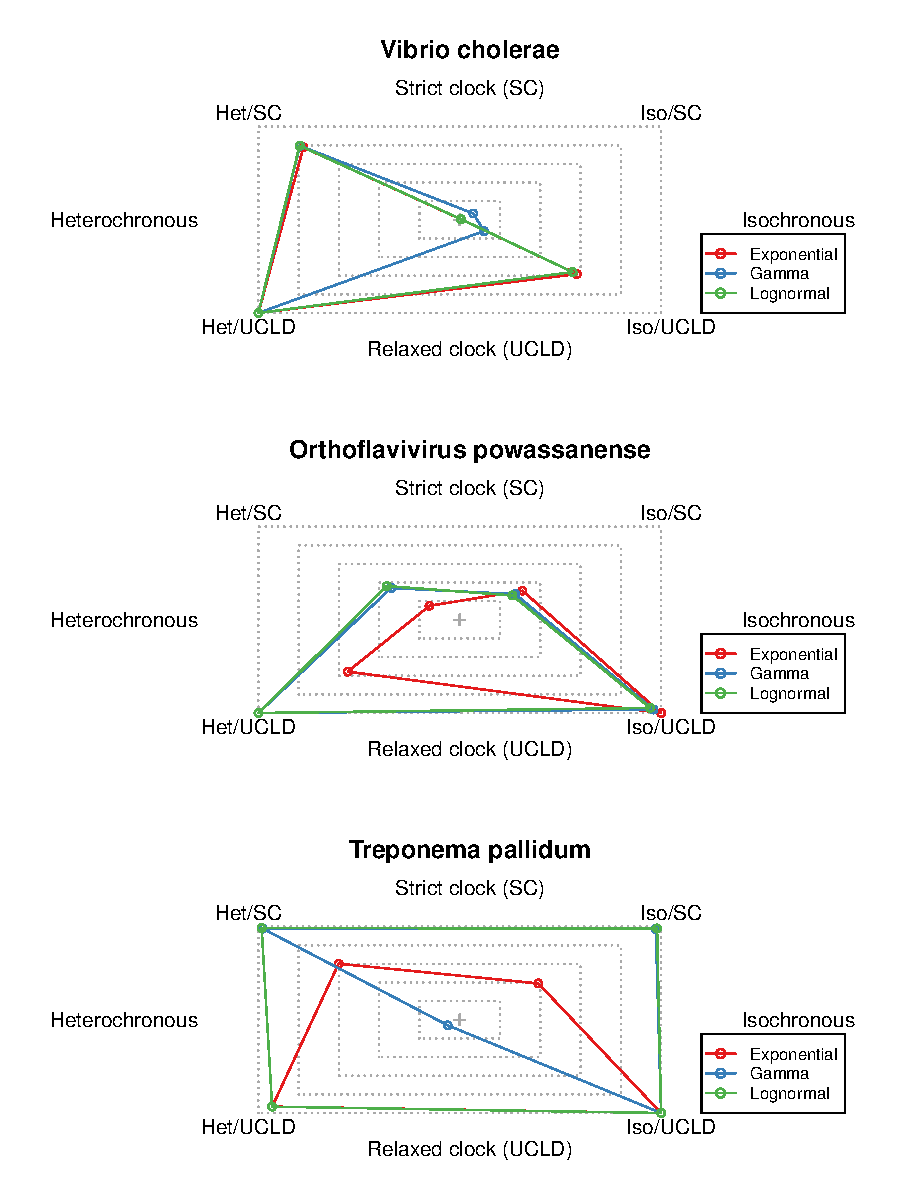
\includegraphics[width=14cm]{sandbox_figures/polygon_plot.pdf}\newline
		\vspace{-0.5cm}
		\caption{\textbf{Relative log marginal likelihoods of empirical data sets}. The polygons represent the relative log marginal likelihoods of each microbe dataset under a different effective population size ($\Phi$) prior, analysed with four different configurations. Het (heterochronous) includes sampling, while iso (isochronous) does not include any sampling times. SC is strict clock and UCLD is the uncorrelated lognormal relaxed clock. Red represents an exponential hyperprior on the effective population size, blue is a $\Gamma$ hyperprior, and green is a log-normal hyperprior.}
		\label{figure:polygon_plots}
	\end{center}
\end{figure}

Our empirical data analyses overall demonstrate that the choice of prior has an impact on Bayesian model selection and support. The \textit{V. cholerae} data set had a posterior that was less sensitive to the prior for key parameters, such as the evolutionary rate (Supplementary material), and in this data set the detection of temporal signal was also more robust to the prior. Moreover, this data set has been shown to have clear clocklike behaviour in root-to-tip regressions and date randomisation tests \cite{duchene2016genome}. In contrast, the data sets of \textit{Powassan virus} and \textit{T. pallidum}, where temporal signal was not supported for all model configurations, we found that the posterior is more sensitive to the choice of prior (). \textcolor{red}{include the density figs as main text}

\subsection*{Simulation experiments}
To understand the impact of the prior on Bayesian model selection we conducted a set of simulation experiments where the data generating process is well understood. We conducted simulations under four possible conditions; a strict or relaxed molecular clock, and where the phylogenetic time-trees were heterochronous or isochronous. Data from heterochronous trees are sampled from a measurably evolving population and are expected to display temporal signal, whereas those from isochronous trees are not from a measurably evolving population (the time-trees are ultrametric) and should not display temporal signal. 

For data generated under heterochronous time-trees, we found that ten out of ten simulation replicates were correctly classified as having temporal signal, using a log Bayes factor of at least 3.2 (Table \ref{table:heterochronous_simulations_unbounded} and Fig \ref{figure:heterochronous_polygons}). This perfect classification was supported regardless of the prior on $\Phi$ and the molecular clock model. 

\begin{table}[h!]
	\caption{\textbf{Correctly classified simulation replicates under heterochronous trees.} A total of ten simulations were generated in each case, under heterochronous trees, such that they are expected to display temporal signal. A number of ten represents perfect classification according to the Bayesian evaluation of temporal signal, BETS and a log Bayes factor of at least 3.2 (strong evidence for temporal signal). The rows correspond to three possible priors on the effective population size of the constant-size coalescent, $\Phi$. The `Best clock model' is a situation where we consider the best heterochronous and isochronous model, take their log Bayes factor, and determine temporal signal if it is at least 3.2.}
	\begin{center}
		\label{table:heterochronous_simulations_unbounded}
		\begin{tabular}{| c + c | c | c |}
			\hline
			\multicolumn{1}{|c|}{\bf True clock model; clock model in analysis} & Exponential & $\Gamma$ & Log-normal\\ \thickhline
			Strict clock; Strict clock     & 10 & 10 & 10 \\ \hline
			Strict clock; Relaxed clock    & 10 & 10 & 10 \\ \hline
			Strict clock; Best clock model & 10 & 10 & 10 \\ \hline
			Relaxed clock; Strict clock    & 10 & 10 & 10 \\ \hline
			Relaxed clock; Relaxed clock    & 10 & 10 & 10 \\ \hline
			Relaxed clock; Best clock model & 10 & 10 & 10 \\ \hline		
		\end{tabular}
	\end{center}
\end{table}

\begin{figure}[!h]
	\begin{center}
		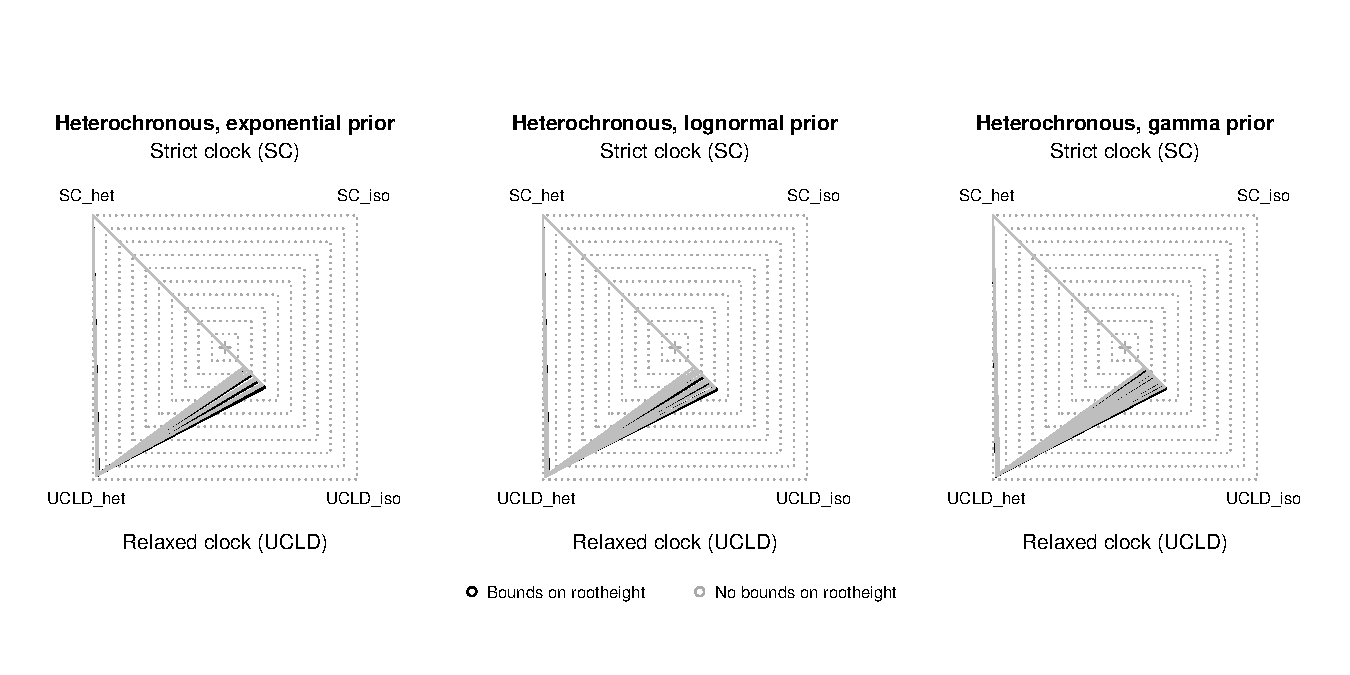
\includegraphics[width=14cm]{sandbox_figures/het_sims.pdf}\newline
		\vspace{-0.5cm}
		\caption{\textbf{Relative log marginal likelihoods of simulations with temporal signal.} The polygons represent the relative log marginal likelihood under three possible priors on the effective population size ($\Phi$) parameter of the constant-size coalescent tree prior. Each corner corresponds to a combination of model and sampling times, either a strict (SC) or relaxed molecular clock with an underlying log-normal distribution (UCLD), and with (heterochronous) or without (isochronous) sampling times. The correct model used to generate the data is the SC heterochronous. Each polygon is for one simulation replicate (a total of ten) and the colours denote whether we employed a hard bound on the root height of the form Uniform(0.0, 5.0) or not.} 
		\label{figure:heterochronous_polygons}
	\end{center}
\end{figure}

For our data generated under isochronous trees, which by definition have no temporal signal, we found perfect classification under the exponential prior on $\Phi$ under both clock models (Table \ref{table:isochronous_simulations_unbounded} and Fig \ref{figure:ultrametric_polygons}). For most analyses under the $\Gamma$ and log-normal priors on $\Phi$ we found that BETS incorrectly supported the presence of temporal signal. The exceptions were for analyses of data analysed under a relaxed clock, whether they were simulated under a strict or relaxed clock. 

A perplexing result occurs under the best molecular clock model for the $\Gamma$ and log-normal priors on $\Phi$. Here we take the log Bayes factor of the best heterochronous model vs the best isochronous model, which produced an increase in the classification error, relative to using the relaxed clock only. This phenomenon occurs because the incorrect inclusion of sampling times can mislead molecular clock model selection. As a case in point one of the simulation replicates under a relaxed molecular clock and an isochronous tree (with no temporal signal) had the following log marginal likelihoods; -4109.87 for the heterochronous analyses with a strict clock, -4117.06 for the isochronous analyses with a strict clock, -4124.35 for the heterochronous analyses with a relaxed clock, and -4118.29 for the isochronous analyses with a relaxed clock. The log Bayes factors under the relaxed clock have strong evidence against temporal signal (log Bayes factor=-6.06 for heterochronous vs isochronous), whereas the opposite is true for the strict clock (log Bayes factor=7.19). However, the best heterochronous model has substantially stronger support than the best isochronous model (here the strict or relaxed molecular clock, whose log marginal likelihoods differ by only 1.3 units). It is also worthwhile to note that in general, analyses under the relaxed clock tended to have fewer classification errors (for data sets with no temporal signal) than the strict clock, regardless of the true molecular clock model used to generate the data.

\begin{table}[h!]
	\caption{\textbf{Correctly classified simulation replicates under isochronous trees.} A total of ten simulations were generated in each case, under isochronous trees, such that they are not expected to support temporal signal. A number of ten represents perfect classification according to the Bayesian evaluation of temporal signal, BETS and a log Bayes factor of at most -3.2 (strong evidence against temporal signal). The rows correspond to three possible priors on the effective population size of the constant-size coalescent, $\Phi$. The `Best clock model' is a situation where we consider the best heterochronous and isochronous model, take their log Bayes factor, and determine a lack of temporal signal if it is at most -3.2.}
	\begin{center}
		\label{table:isochronous_simulations_unbounded}
		\begin{tabular}{| c + c | c | c |}
			\hline
			\multicolumn{1}{|c|}{\bf True clock model; clock model in analysis} & Exponential & $\Gamma$ & Log-normal\\ \thickhline
			Strict clock; Strict clock     & 10 & 0 & 0 \\ \hline
			Strict clock; Relaxed clock    & 10 & 10 & 10 \\ \hline
			Strict clock; Best clock model & 10 & 0 & 0 \\ \hline
			Relaxed clock; Strict clock    & 10 & 0 & 0 \\ \hline
			Relaxed clock; Relaxed clock    & 10 & 9 & 9 \\ \hline
			Relaxed clock; Best clock model& 10 & 0 & 1 \\ \hline		
		\end{tabular}
	\end{center}
\end{table}

\begin{figure}[!h]
	\begin{center}
		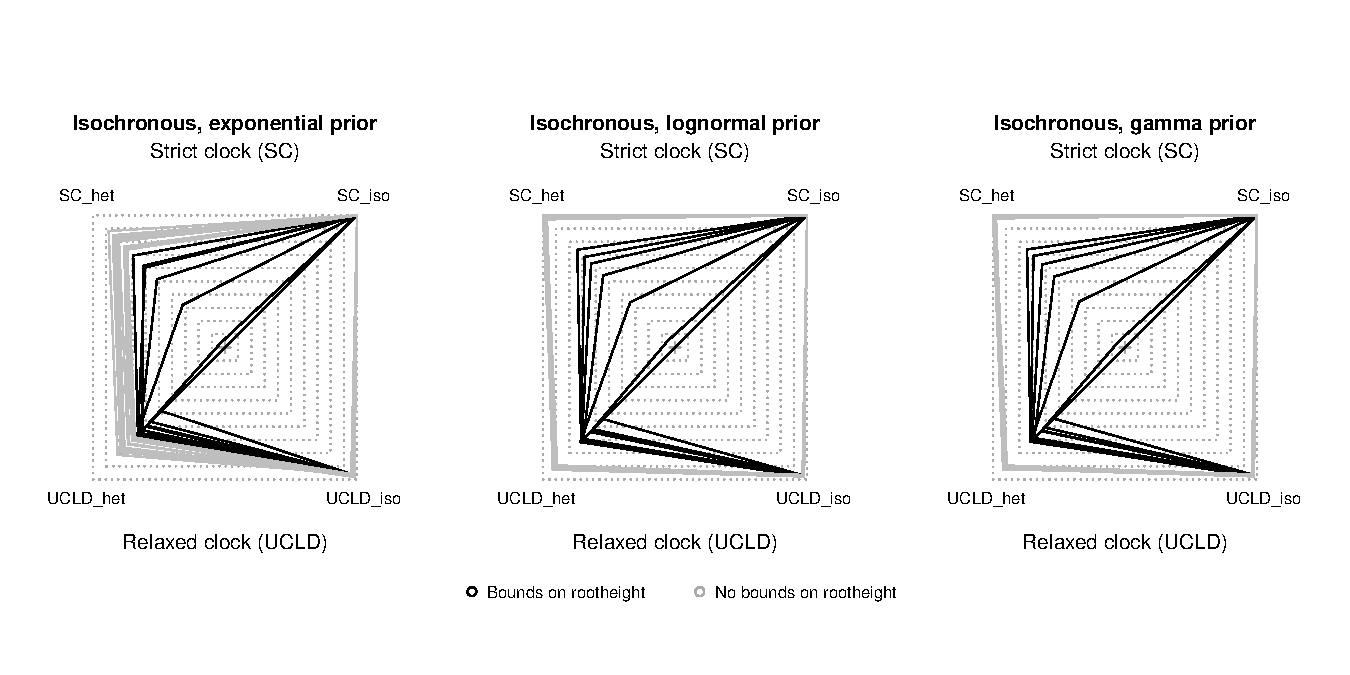
\includegraphics[width=14cm]{sandbox_figures/iso_sims.pdf}\newline
		\vspace{-0.5cm}
		\caption{\textbf{Relative log marginal likelihoods of simulations with no temporal signal.} The polygons here represent the same information as in Fig \ref{figure:heterochronous_polygons}. The correct model used to generate the data here is the SC isochronous (ultrametric).} 
		\label{figure:ultrametric_polygons}
	\end{center}
\end{figure}

Our simulation results demonstrate that detecting temporal signal when it is not present, which is akin to a type I error, is more common under some prior configurations (here the $\Gamma$ and log-normal priors on $\Phi$) than the opposite (failing to detect temporal signal when it is present). Upon inspecting the resulting phylogenetic trees and the posterior of key parameters we found a probable cause. The incorrect inclusion of sampling times produces a dramatic overestimate of the height of the tree, especially under the strict molecular clock model (Fig \ref{figure:ultrametric_tree_distortion}). Under this situation, the sampling times represent such a small proportion of the tree height, that the heterochronous tree is indistinguishable from one that is ultrametric and thus their log marginal likelihoods can be similar. In fact, the inclusion of sampling times may improve the fit of the model by accommodating natural stochasticity in the root-to-tip distances. The phenomenon of tree extension also occurs under the relaxed molecular clock, but to a much lesser extent, such that under this model it is easier to correctly classify isochronous data sets. The exponential tree prior favour shallower trees and this is probably the reason for why results in more accurate classification.

\begin{figure}[h!]
	\begin{center}
		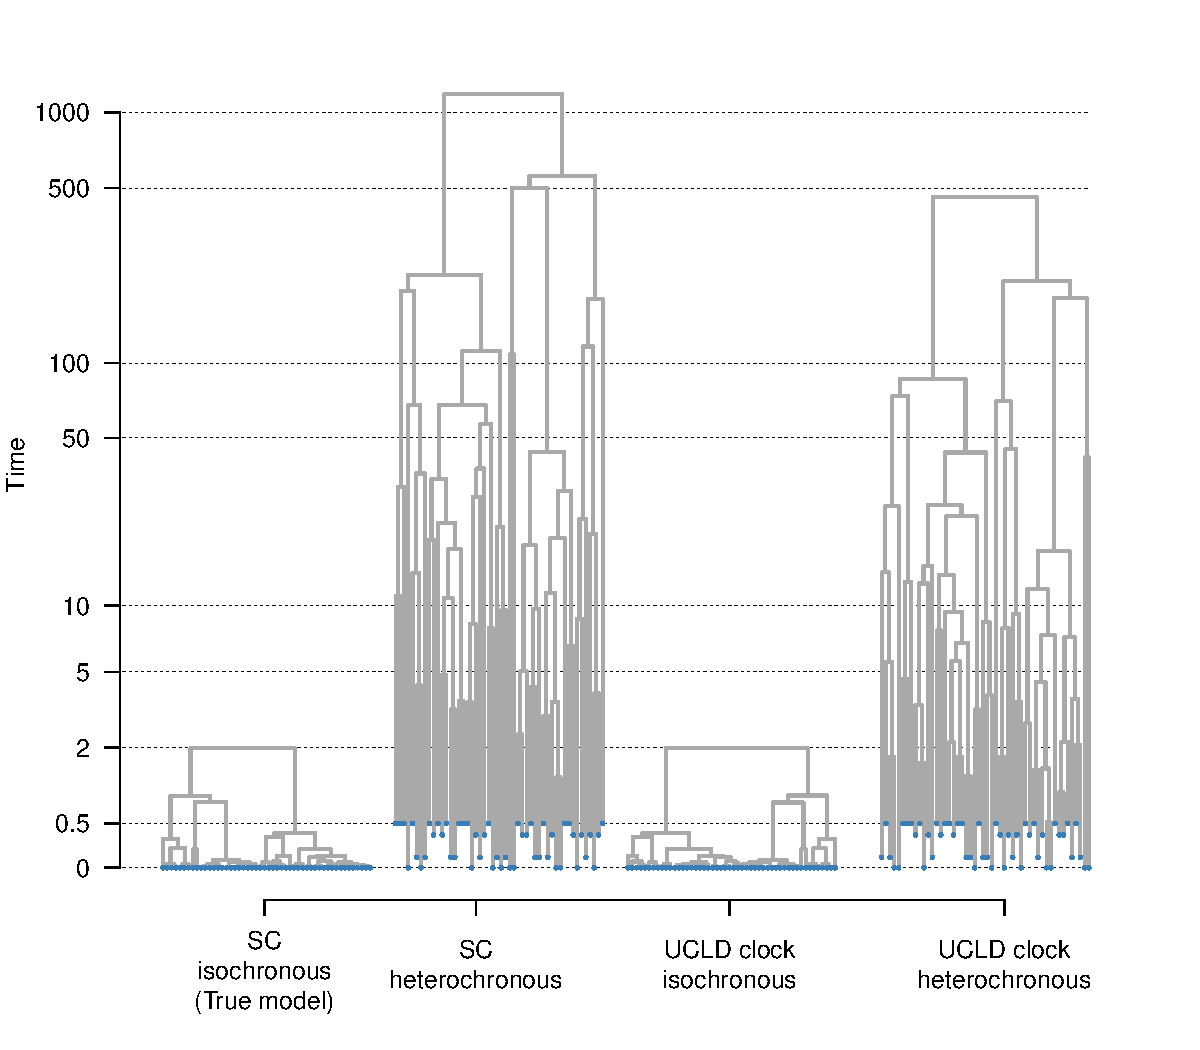
\includegraphics[width=15cm]{sandbox_figures/tree_distortion_ultrametric.pdf}\newline
		\vspace{-0.5cm}
		\caption{\textbf{Distortion of phylogenetic node times from a simulation replicate with no temporal signal}. Highest clade credibility trees from a data set simulated with no sampling times (isochronous) and under a strict molecular clock model (SC). The prior on $\Phi$ is a $\Gamma(\kappa=0.001, \theta=1000)$, which resulted in high classification errors. Tip nodes are labelled with solid blue circles. Including sampling times that span 0.5 units of time and about 1/4 of the true tree height induces dramatic overestimation of the tree height. This effect occurs under the SC and the relaxed molecular clock with an underlying log-normal distribution (UCLD), but it is markedly less pronounced in the UCLD. Note that the y-axis is in logarithmic scale (log$_{10}$).}
		\label{figure:ultrametric_tree_distortion}
	\end{center}
\end{figure}

In Fig \ref{figure:heterochronous_tree_distortion} we show an example of phylogenetic trees from a simulation replicate with temporal signal (heterochronous). Failing to include sampling times, as in isochronous analyses, results in trees that are of similar height, so the confounding effect that we observe in isochronous data sets above does not occur. However, the time-scale of the isochronous trees is determined by the value used to fix the molecular clock rate. The typical approach is to fix this parameter to 1.0, which means that genetic distance and time are the same. A problem with this method is that the $\Phi$ parameter of the constant-size coalescent is proportional to units of time \cite{ho2011skyline, drummond2002estimating} (as are most other parameters of the tree prior, for example the growth rate of the exponential-growth coalescent). Thus, the prior on $\Phi$ for the heterochronous and isochronous analyses has different meanings, unless this parameter is scaled to match the units of the branch lengths, or the molecular clock rate in the isochronous analyses is fixed to a plausible value. In our simulations we fixed the molecular clock rate to its true value, but we also found that using a number within the expected order of magnitude of the organism in question is sufficient (e.g. 10$^{-4}$ to 10$^{-3}$ subs/site/year for a ssRNA virus).

\begin{figure}[!h]
	\begin{center}
		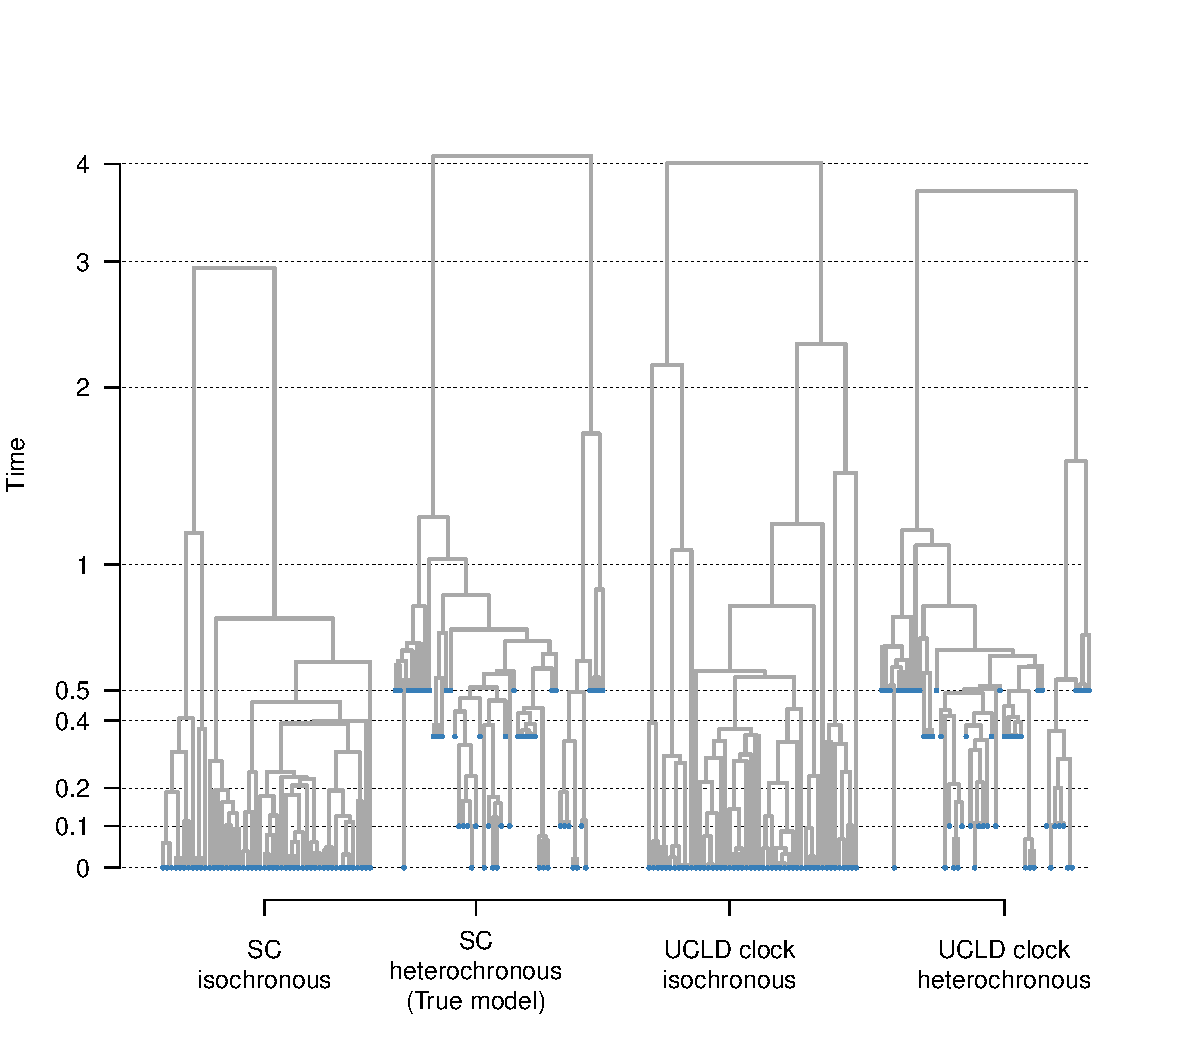
\includegraphics[width=15cm]{sandbox_figures/tree_distortion_heterochronous.pdf}\newline
		\vspace{-0.5cm}
		\caption{\textbf{Distortion of phylogenetic node times from a simulation replicate with temporal signal}. Highest clade credibility trees from a data set simulated with sampling times (heterochronous) and under a strict molecular clock model (SC). The isochronous trees are inferred by fixing the molecular clock rate to the true value, such that the time-scale is in the comparable units to the heterochronous analyses. Unlike the estimates for isochronous trees (e.g. Fig \ref{figure:ultrametric_tree_distortion}), the root height of the trees with under all scenarios are comparable. Axes and labels are the same as those of Fig \ref{figure:ultrametric_tree_distortion}}
		\label{figure:heterochronous_tree_distortion}
	\end{center}
\end{figure}


Defining a suitable prior for the parameters of the tree prior requires careful attention. The prior on $\Phi$ (or other parameters) should not favour implausibly node heights. However, understanding the interplay between the parameters of the tree prior and the resulting tree topologies and node heights is not necessarily trivial, particularly when the tree prior involves multiple parameters (e.g. the Bayesian skyride). A pragmatic solution is to include additional prior information in the form of hard bounds on the root-height or the molecular clock rate. To this end, we investigated the effect of including a uniform prior between 0.0 and 5.0 units of time for the tree height, meaning that trees that are older than 5.0 units have a prior probability of 0.0. Importantly, the trees under which we generated our simulations had root heights of around 2.0 units of time, and thus the hard bound of 5.0 allows for trees that are over twice as old as the truth. 

Setting hard bounds on the root height resulted in perfect classification accuracy for both, the heterochronous and isochronous simulation (Table \ref{table:heterochronous_simulations_bounded} and Fig \ref{figure:heterochronous_polygons}, and Table \ref{table:isorochronous_simulations_bounded} and Fig \ref{figure:ultrametric_polygons}, respectively). The improvement in classification for data sets with no temporal signal is likely because the hard bounds limit the tree extension phenomenon and thereby including sampling times imposes a penalty on the log marginal likelihood (see polygons in Fig \ref{figure:heterochronous_polygons}).

\begin{table}[h!]
	\caption{\textbf{Correctly classified simulation replicates under heterochronous trees using hard bounds on the root height.} Rows and columns are identical to those of Table \ref{table:heterochronous_simulations_unbounded}, but here the heterochronous analyses include an explicit prior on the root height, via a uniform distribution between 0 and 5.0.}
	\begin{center}
		\label{table:heterochronous_simulations_bounded}
		\begin{tabular}{| c + c | c | c |}
			\hline
			\multicolumn{1}{|c|}{\bf True clock model; clock model in analysis} & Exponential & $\Gamma$ & Log-normal\\ \thickhline
			Strict clock; Strict clock     & 10 & 10 & 10 \\ \hline
			Strict clock; Relaxed clock    & 10 & 10 & 10 \\ \hline
			Strict clock; Best clock model & 10 & 10 & 10 \\ \hline
			Relaxed clock; Strict clock    & 10 & 10 & 10 \\ \hline
			Relaxed clock; Relaxed clock    & 10 & 10 & 10 \\ \hline
			Relaxed clock; Best clock model & 10 & 10 & 10 \\ \hline		
		\end{tabular}
	\end{center}
\end{table}

\begin{table}[h!]
	\caption{\textbf{Correctly classified simulation replicates under isochronous trees using hard bounds on the root height.} Rows and columns are identical to those of Table \ref{table:isochronous_simulations_unbounded}, but here the heterochronous analyses include an explicit prior on the root height, via a uniform distribution between 0 and 5.0.}
	\begin{center}
		\label{table:isorochronous_simulations_bounded}
		\begin{tabular}{| c + c | c | c |}
			\hline
			\multicolumn{1}{|c|}{\bf True clock model; clock model in analysis} & Exponential & $\Gamma$ & Log-normal\\ \thickhline
			Strict clock; Strict clock     & 10 & 10 & 10 \\ \hline
			Strict clock; Relaxed clock    & 10 & 10 & 10 \\ \hline
			Strict clock; Best clock model & 10 & 10 & 10 \\ \hline
			Relaxed clock; Strict clock    & 10 & 10 & 10 \\ \hline
			Relaxed clock; Relaxed clock    & 10 & 10 & 10 \\ \hline
			Relaxed clock; Best clock model& 10 & 10 & 10 \\ \hline		
		\end{tabular}
	\end{center}
\end{table}

\subsection*{Prior predictive simulations and parameter correlations}
\textcolor{red}{Two points here, first that there exist correlations between parameters, which should be investigated (show plots of parameter correlations). Second that the prior can be easily investigated, for example to know what the prior on the root height is, when it is not explicit (show root prior and trees for simulations).}

\begin{table}[!ht]
\begin{adjustwidth}{-2.25in}{0in}
\centering
\caption{
{\bf Proportion of simulations with temporal signal under heterochronous simulated data}}
\begin{tabular}{ | c + c | c | c | c | }
\hline
\multicolumn{1}{|c|}{\bf Species; Clock Model} & Exponential & Gamma & Lognormal \\ \thickhline
\hline
$Vibrio$ $cholerae;$ $Strict$ $Clock$ & 10 & 10 & 10 \\ \hline
$Vibrio$ $cholerae;$ $Relaxed$ $Clock$ & 10 & 10 & 10 \\  \hline
$Vibrio$ $cholerae;$ $Best\ clock\ model$ & 10 & 10 & 10 \\  \hline
$Orthoflavivirus$ $powassanense;$ $Strict$ $Clock$ &  &  &  \\ \hline
$Orthoflavivirus$ $powassanense;$ $Relaxed$ $Clock$ &  &  &  \\  \hline
$Treponema$ $pallidum;$ $Strict$ $Clock$ & 0 & 0 & 0 \\ \hline
$Treponema$ $pallidum;$ $Relaxed$ $Clock$ & 0 & 10 & 8 \\ \hline
$Treponema$ $pallidum;$ $Relaxed$ $Clock$ & & & \\ \hline
\end{tabular}
\end{adjustwidth}
\end{table}

\begin{table}[!ht]
\begin{adjustwidth}{-2.25in}{0in}
\centering
\caption{
{\bf Proportion of simulations without temporal signal under isochronous simulated data}}
\begin{tabular}{ | c + c | c | c | c | }
\hline
\multicolumn{1}{|c|}{\bf Species; Clock Model} & Exponential & Gamma & Lognormal \\ \thickhline
\hline
$Vibrio$ $cholerae;$ $Strict$ $Clock$ & 10 & 0 & 0 \\ \hline
$Vibrio$ $cholerae;$ $Relaxed$ $Clock$ & 0 & 0 & 0 \\  \hline
$Vibrio$ $cholerae;$ $Best\ clock\ model$ & 0 & 0 & 0 \\  \hline
$Orthoflavivirus$ $powassanense;$ $Strict$ $Clock$ &  &  &  \\ \hline
$Orthoflavivirus$ $powassanense;$ $Relaxed$ $Clock$ &  &  &  \\  \hline
$Treponema$ $pallidum;$ $Strict$ $Clock$ & 10 & 10 & 10 \\ \hline
$Treponema$ $pallidum;$ $Relaxed$ $Clock$ & 10 &  0 &  0 \\ \hline
$Treponema$ $pallidum;$ $Best\ clock\ model$ & &  &  \\ \hline
\end{tabular}
\end{adjustwidth}
\end{table}



\textcolor{red}{To do: Plot densities of clock rates, root height, tree length, coefficient of rate variation. One panel per data set, show density for the three priors and the same colours as the fig above.}
            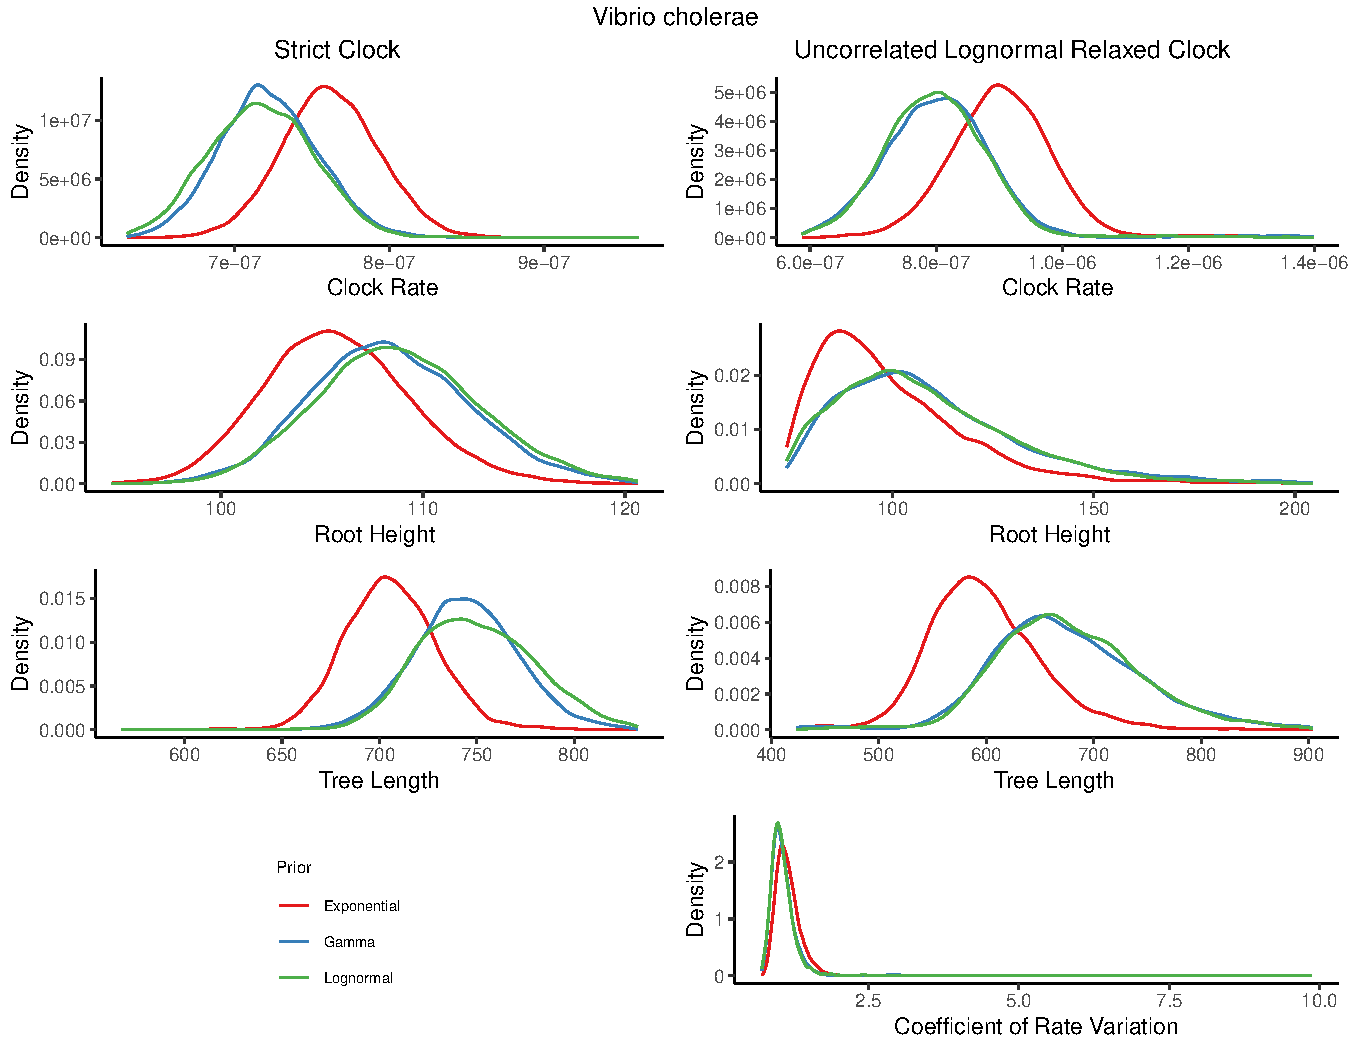
\includegraphics[width=13cm]{sandbox_figures/cholera_density_plot.pdf}\newline
            Density plots of the clock rate, root height, tree length, and coeffcient of rate variation of cholera.
            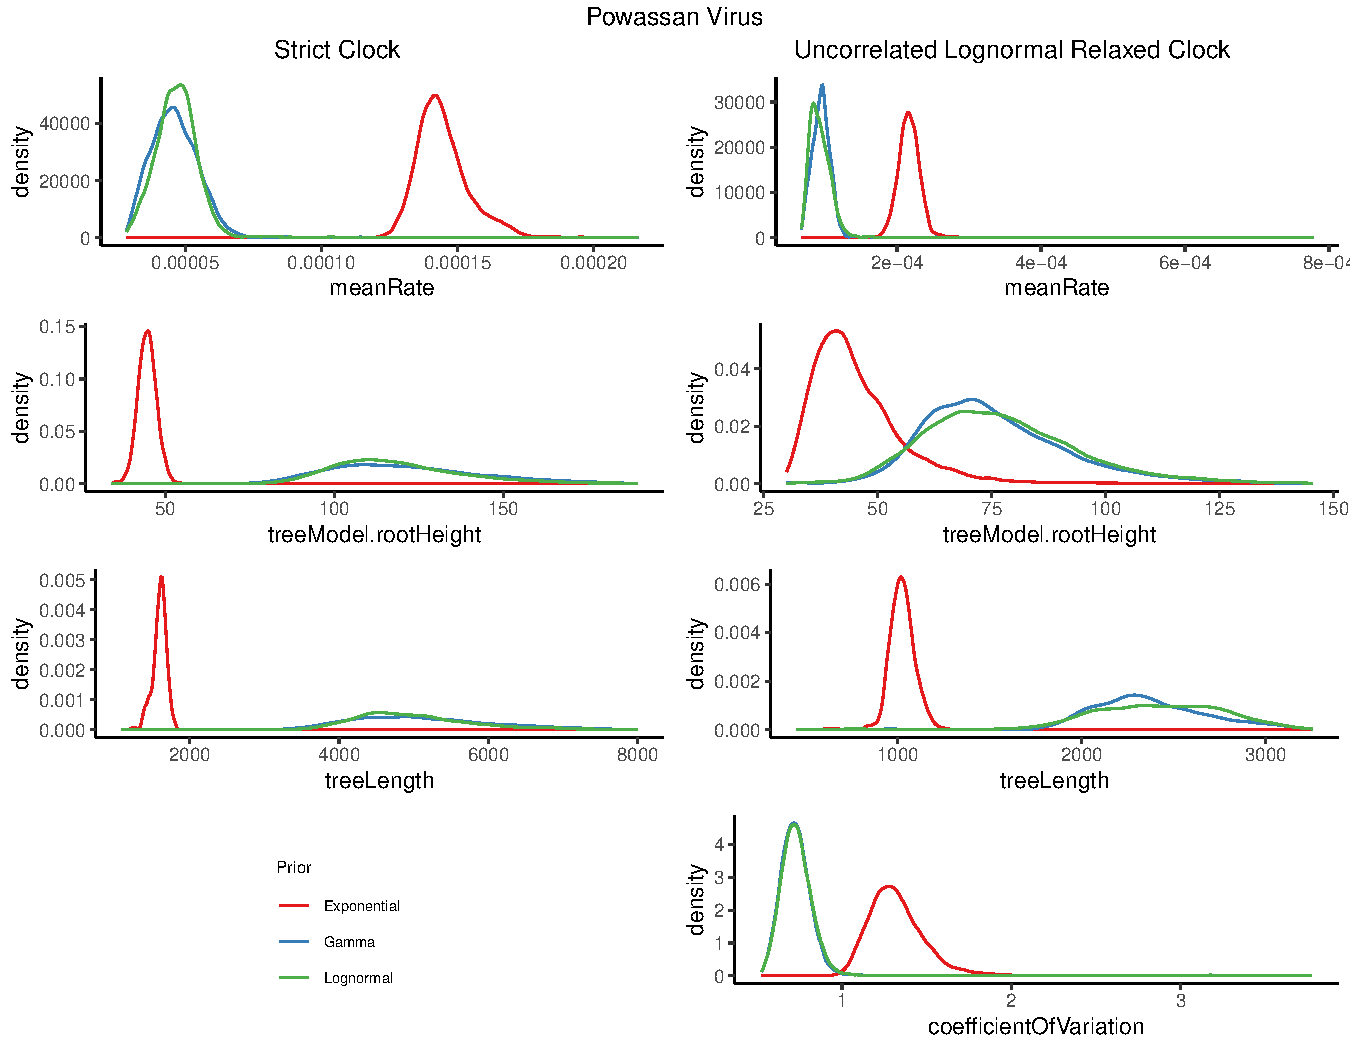
\includegraphics[width=13cm]{sandbox_figures/powv_density_plot.pdf}\newline
            Density plots of the clock rate, root height, tree length, and coeffcient of rate variation of powassan virus.
            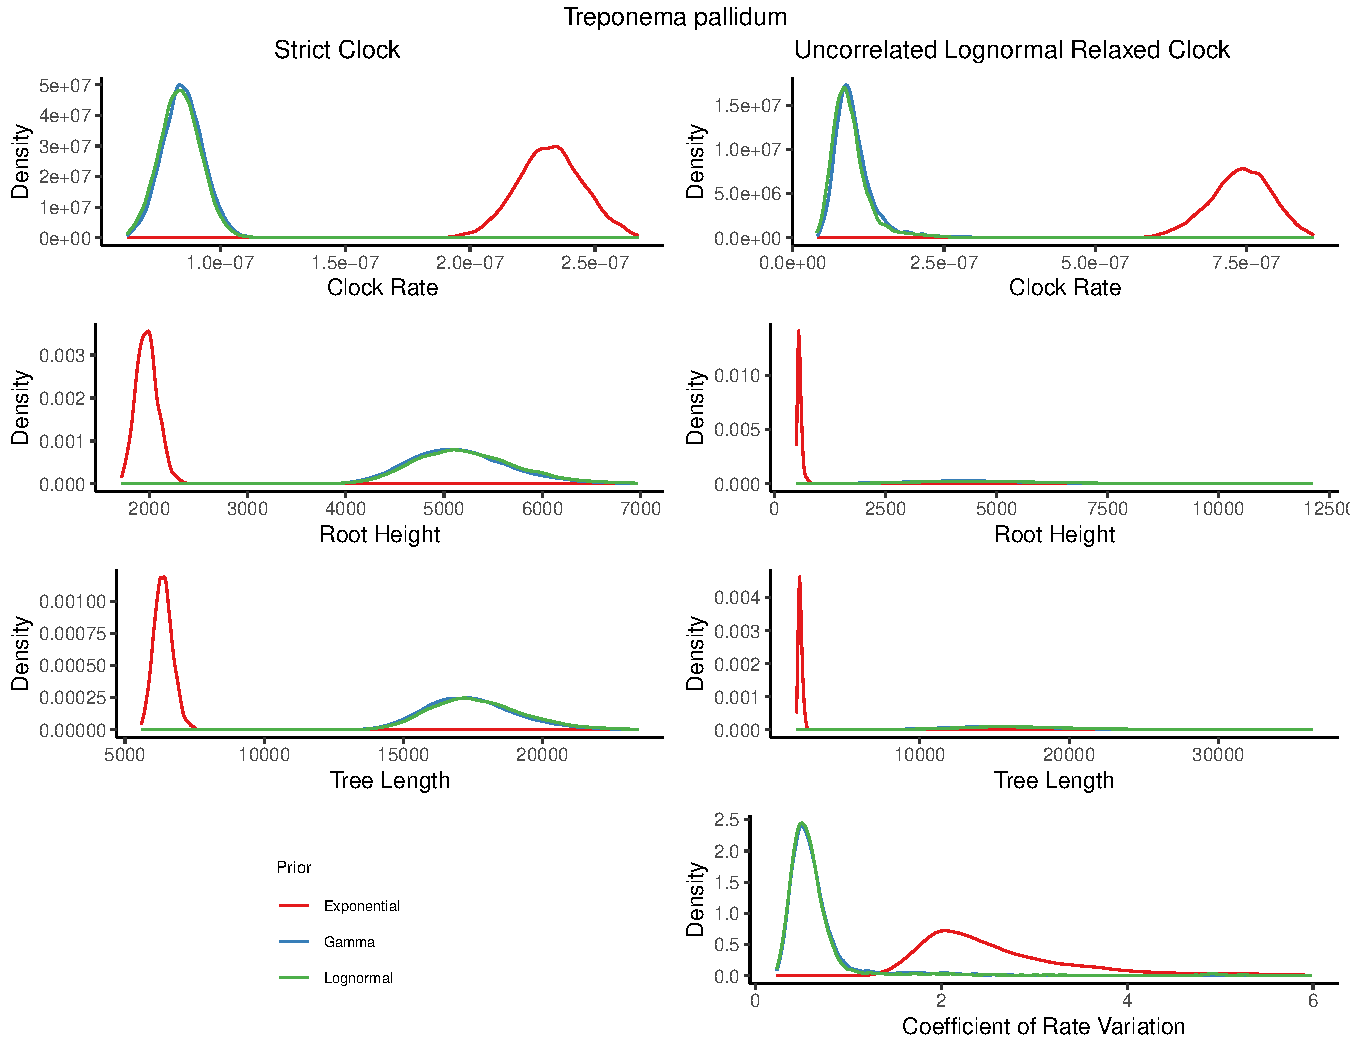
\includegraphics[width=13cm]{sandbox_figures/treponema_density_plot.pdf}\newline
            Density plots of the clock rate, root height, tree length, and coeffcient of rate variation of treponema palladium.





\section*{Discussion}

\textcolor{red}{
Whole genome sequencing and ancient DNA are two technologies that have dramatically expanded the range of organisms from which we can sample measurably evolving populations. By sequencing complete genomes, instead of individual genes, we can capture more genetic variation overall. In a microbe with an evolutionary rate of about 1$\times 10^{-7}$ subs/site/year (e.g. \textit{M. tuberculosis} \cite{menardo2019molecular}) sampled over a decade would yield on average one substitution for every 1M bases sequenced, with shorter stretches of sequences being mostly uninformative. As a result, many microbes whose evolution was considered too slow to be treated a measurably evolving populations, including many bacteria, are now commonly analysed using frameworks that were thought to be only applicable to rapidly evolving pathogens, such as RNA viruses \cite{biek2015measurably}.}

\textcolor{red}{Ancient DNA has had a profound impact in our understanding of the long-term evolution of many microbial pathogens \cite{duchene2020recovery,spyrou2019ancient}. The inclusion of ancient DNA in molecular evolutionary analyses can substantially broaden the sampling window, and therefore provide invaluable data points for molecular clock calibration because the data can effectively be treated as coming from a measurably evolving population \cite{ho2020dating}.}

\textcolor{red}{Remember to mention the book chapter where we also look at how the prior on root height is affected by the presence or absence of temporal signal. Data sets with temporal signal should see more distance between the prior and the posterior. }

\section*{Materials and methods}
\subsection*{Empirical data}
We selected three different datasets to evaluate temporal signal, cholera (), powassan virus (), and treponema (). These varied in their timespans, number of informative sites, and number of sequences. The most sparse dataset was treponema, where sampling dates spanned 481 years, with 28 sequences each containing 1500 sites. There were 319 sequences with 11193 sites for powassan virus, spanning 5 years of sampling times. Finally, we had 122 cholera sequences with 1757 sites across 73 years of sampling.
For the empirical data there are 1392 unique site patterns in cholera, 3457 in powassan virus, and 840 in treponema. In the simulated data, there are 580-710 (SC) and 640-710 (UCLD) in cholera, there are 110-150 in both SC and UCLD for treponema. For the powassan virus SC, there are $\sim$4800 in the isochronous trees and $\sim$14650 in the heterchronous trees.

\begin{table}[h]
\caption{Unique Site Patterns for each dataset and clock model}
\begin{center} 
	\label{table:prior_distros_on_Phi}
	\begin{tabular}{| c + c | c | c |}
    \hline
		\multicolumn{1}{|c|}{Dataset} & Empirical & Simulation (SC) & Simulations (UCLD) \\ \thickhline
		Cholera & 1392 & 580-710 & 640-710\\ \hline
        Powassan Virus & 3457 & $\sim$4800 (iso) & $\sim$14650 (het)\\ \hline
		Treponema & 840 & 110-150 & 110-150\\ \hline
	\end{tabular}
\end{center}
\end{table}

We sampled the posterior distribution using Markov chain Monte Carlo as implemented in BEAST1.10. The chain length was $10^{8}$ steps, sampling every $10^3$ to draw a total of $10^4$ samples. The prior for the evolutionary rate of the strict clock was a CTMC rate reference prior (i.e. a $\Gamma(\alpha=0.5, \beta=T$, with $T=$ tree length, and mean=$\alpha/\beta$). For the log-normal distribution of the relaxed clock we also used the CTMC rate reference prior for the mean rate (known as the ucld.mean in the program) and an exponential prior with mean 0.33 for the standard deviation (the ucld.stdev in the program). For the tree prior we used a constant-size coalescent with population size, $\Phi$ with three possible priors, as described in Table \ref{table:prior_distros_on_Phi}. In all cases we used the HKY+$\Gamma_4$ substitution model, with the default priors in BEAST1.10.

To calculate log marginal likelihoods we used generalised stepping-stone \cite{baele2016genealogical,fan2011choosing}. This method requires a working distribution for all parameters, including the tree prior, for which we used the matching coalescent model. We set 100 path steps between the unnormalised posterior and the working distribution, following equally spaced intervals from a $\beta(0.3, 1.0)$ distribution. For each step we ran a chain length of 2$\times 10^{6}$ steps.

\subsection*{Simulation experiments}
\textcolor{red}{Sebastian, describe small simulations. That is, that the population size was 1.0, and what the clock rates were. For the analyses say that in the isochronous the clock rate was fixed to the correct value to ensure that the units are correct, etc... Also describe how we designed the bounds here and what they do}



\section*{Supporting information}

% Include only the SI item label in the paragraph heading. Use the \nameref{label} command to cite SI items in the text.
\paragraph*{S1 Fig.}
\label{S1_Fig}
{\bf Bold the title sentence.} Add descriptive text after the title of the item (optional).

\paragraph*{S2 Fig.}
\label{S2_Fig}
{\bf Lorem ipsum.} Maecenas convallis mauris sit amet sem ultrices gravida. Etiam eget sapien nibh. Sed ac ipsum eget enim egestas ullamcorper nec euismod ligula. Curabitur fringilla pulvinar lectus consectetur pellentesque.

\paragraph*{S1 File.}
\label{file:S1_File}
{\bf Lorem ipsum.}  Maecenas convallis mauris sit amet sem ultrices gravida. Etiam eget sapien nibh. Sed ac ipsum eget enim egestas ullamcorper nec euismod ligula. Curabitur fringilla pulvinar lectus consectetur pellentesque.

\section*{Acknowledgments}
This work was supported by the Inception program [Investissement d’Avenir grant ANR-16-CONV-0005], the Australian National Health and Medical Research Council [APP1157586], and the Australian Research Council [DE190100805].

\nolinenumbers

% Either type in your references using
% \begin{thebibliography}{}
% \bibitem{}
% Text
% \end{thebibliography}
%
% or
%
% Compile your BiBTeX database using our plos2015.bst
% style file and paste the contents of your .bbl file
% here. See http://journals.plos.org/plosone/s/latex for 
% step-by-step instructions.
% 
%\begin{thebibliography}{10}
\bibliography{References}

%\bibitem{bib1}
%Conant GC, Wolfe KH.
%\newblock {{T}urning a hobby into a job: how duplicated genes find new
%  functions}.
%\newblock Nat Rev Genet. 2008 Dec;9(12):938--950.

%\bibitem{bib2}
%Ohno S.
%\newblock Evolution by gene duplication.
%\newblock London: George Alien \& Unwin Ltd. Berlin, Heidelberg and New York:
%  Springer-Verlag.; 1970.

%\bibitem{bib3}
%Magwire MM, Bayer F, Webster CL, Cao C, Jiggins FM.
%\newblock {{S}uccessive increases in the resistance of {D}rosophila to viral
%  infection through a transposon insertion followed by a {D}uplication}.
%\newblock PLoS Genet. 2011 Oct;7(10):e1002337.

%\end{thebibliography}



\end{document}

